\section{Introduction}
\label{sec:intro}

On-policy distillation (OPD) is becoming increasingly common in frontier LLM post-training.
Qwen3~\citep{yang2025qwen3}, MiMo~\citep{xiao2026mimo}, GLM-5~\citep{zeng2026glm}, DeepSeek-V4~\citep{xu2026deepseek}, and Kimi K3~\citep{team2026kimi} all use OPD alongside supervised fine-tuning (SFT) and reinforcement learning (RL).
What makes OPD distinctive is its combination of on-policy state visitation and dense distillation supervision~\citep{gu2024minillm,agarwal2024policy}.
The student samples its own rollouts, while the teacher provides the full next-token distribution at every visited prefix, yielding dense, token-level supervision rather than the single outcome-level reward typically used in reinforcement learning with verifiable rewards (RLVR).

A growing line of work has systematically investigated OPD's training dynamics and mechanisms, largely from an algorithmic perspective, to explain how and why the method works~\citep{li2026rethinking,fu2026revisiting,cai2026learning,zhu2026many}.
Yet no prior work has studied how training data shapes OPD, or how the data and the algorithm interact.
Closing this gap is essential to a complete understanding of OPD.
In RLVR, \citet{wang2025oneshot} introduce one-shot RLVR as an extreme controlled experiment to isolate the role of training data.
We bring the same experimental lens to OPD by training on a single query, a setting we call one-shot OPD.
To our surprise, one-shot OPD produces a learning curve strikingly similar to that of one-shot RLVR as shown in Figure~\ref{fig:teaser}: despite repeatedly training on just one query, the model continues to improve for hundreds of steps and ultimately achieves a substantial gain.
We therefore devote this work to answering a single question:

\textit{Why can OPD, when trained on just one example, \textbf{keep learning for so long} and \textbf{improve by so much}?}

\begin{figure}[!ht]
    \centering
    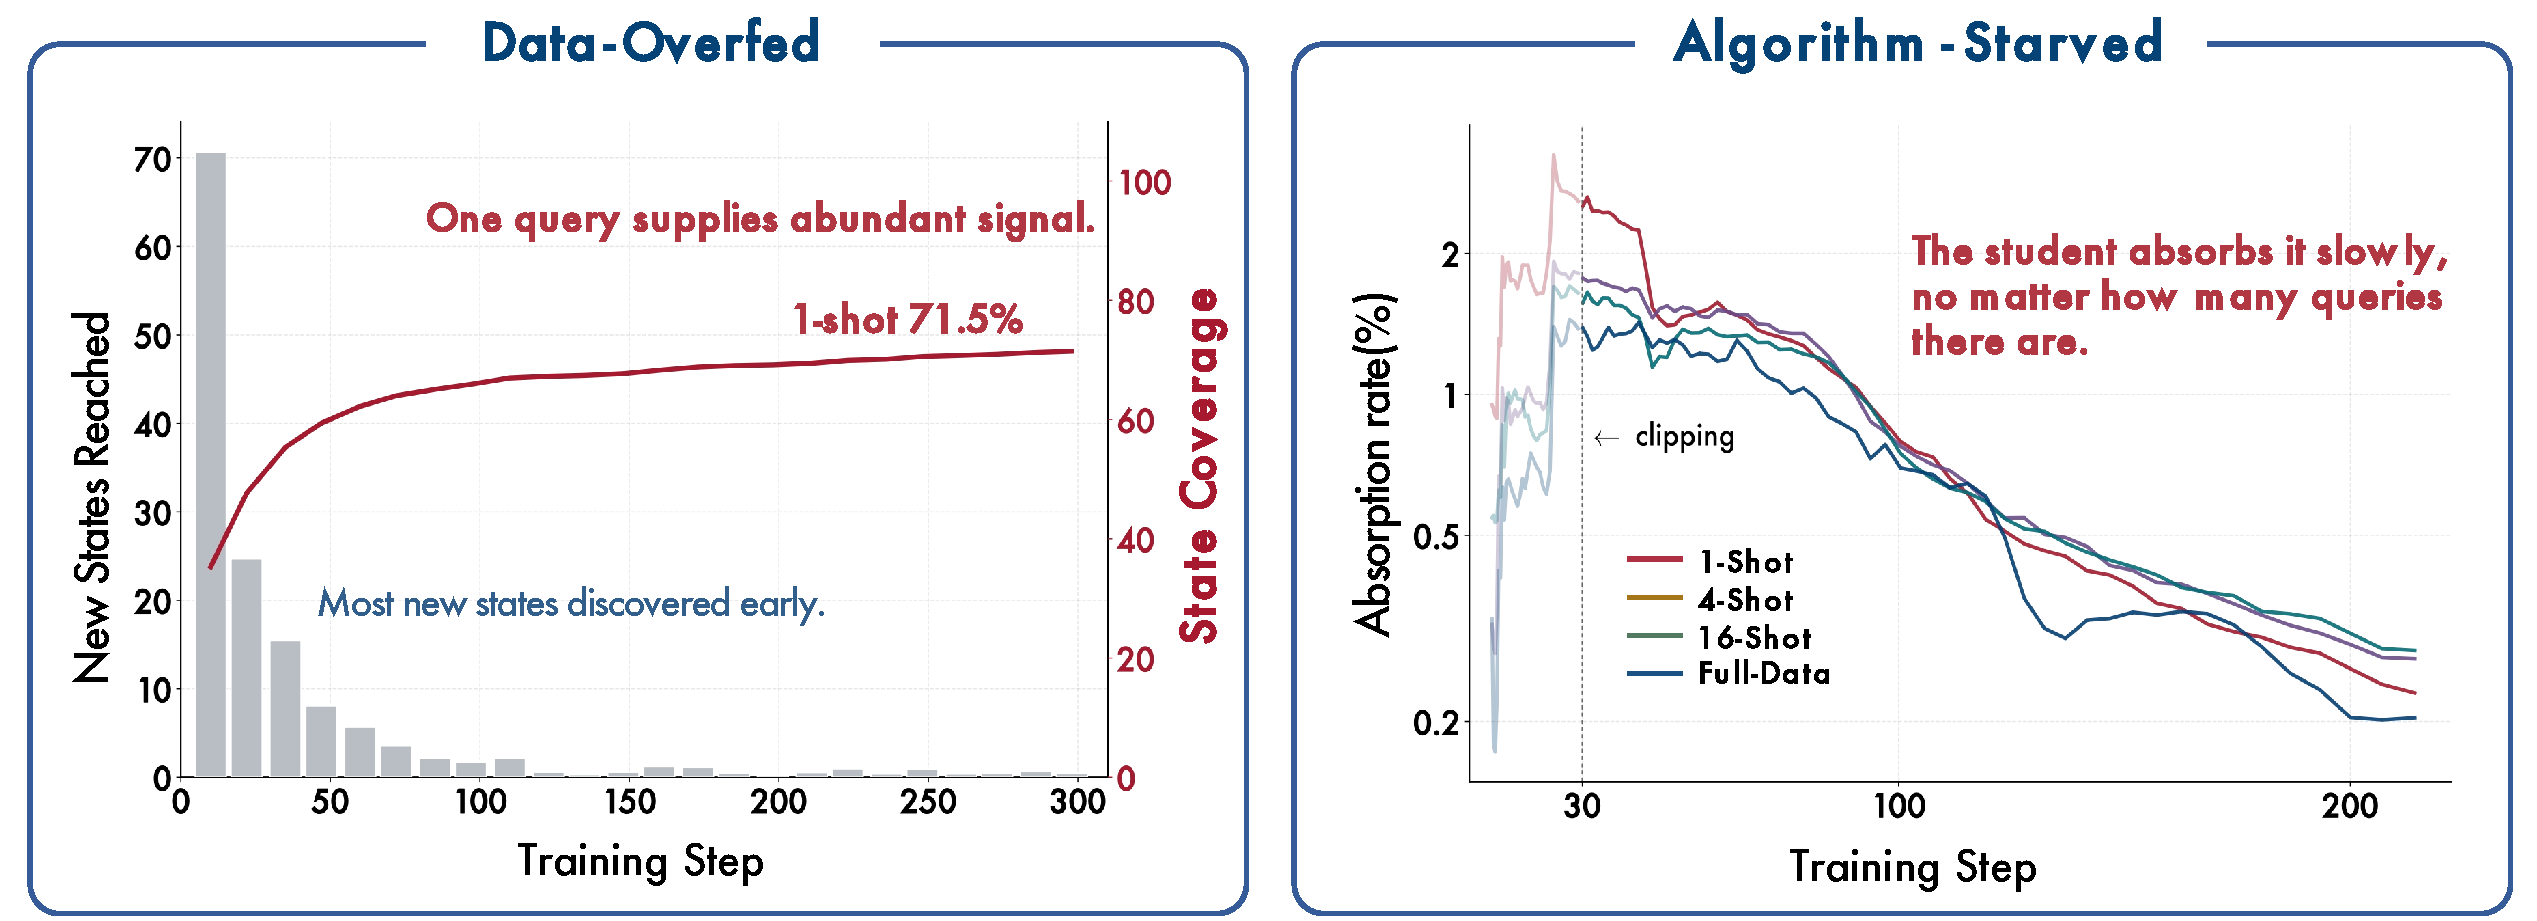
\includegraphics[width=\linewidth]{figures/main2.pdf}
    \caption{\textbf{OPD is data-overfed but algorithm-starved.} \textbf{Data:} one query already covers most of the states full-data OPD visits. \textbf{Algorithm:} the student absorbs an ever smaller proportion of the remaining teacher--student gap, no matter how many queries it trains on.}
    \label{fig:overview}
\end{figure}

This question exposes two aspects of OPD efficiency that standard training entangles:
\textit{\textbf{keep learning for so long}} concerns how fast the \textit{algorithm} absorbs supervision, whereas \textit{\textbf{improve by so much}} concerns why a small amount of \textit{data} supply sufficient supervision.
By reducing the data supply to its minimum, one-shot OPD disentangles the two, and the phenomenon itself proves robust: the gain holds across four task domains and three model families, and persists even on queries the student never solves (\Cref{sec:one-shot}).
Our answer is that \textbf{OPD is data-overfed but algorithm-starved}.
From the \textit{data perspective}, a query acts on the student through the \emph{states} its rollouts reach, each state being a prefix \(s=(x,y_{<i})\) at which the teacher supplies token-level supervision, so a query set is worth the part of that space it covers. We quantify this by \emph{state coverage}: we group the states full-data OPD visits into semantic clusters and report the fraction a setting's rollouts reach. A single query already supplies enough states on its own, covering \(71.5\%\) of what full-data OPD visits, and 16 semantically diverse queries cover \(98.9\%\) and match full-data training (\Cref{sec:data}). This is why so little data improves the student by so much. From the \textit{algorithm perspective}, what falls as training proceeds is the \emph{absorption rate}, the proportion of the remaining teacher--student gap that one update closes, and it declines in much the same way on one query as on all 17k (\Cref{sec:algorithm}), so the pace of a run is a property of OPD rather than of the training set.
In other words, the supervision a single query supplies remains largely unexploited, rate-limited by how quickly an on-policy student can absorb it.

The same mechanism informs data design beyond the one-shot setting.
In multi-teacher OPD (MOPD)~\citep{xiao2026mimo,xu2026deepseek}, where a single student is trained across several domains and each query is routed to its domain teacher, we find that 16 semantically diverse queries per domain suffice to match full-data training (\Cref{sec:mopd}).
Taking the data side to its extreme, we further show that even a training input that states no problem can remain effective: off-domain WildChat prompts and content-free templates drive OPD nearly as effectively as the full training set (\Cref{sec:template}).
Therefore, an input is useful largely because it starts the student reasoning.
Furthermore, we conduct a controlled comparison with one-shot RLVR on the same query to make the algorithmic contrast concrete: the outcome reward is exhausted once the query is solved on nearly every rollout, whereas OPD's token-level signal persists throughout training, and OPD's validation gain over $1000$ steps is more than twice that of RLVR (\Cref{sec:opd-vs-rlvr}).

In short, OPD is supplied with more supervision than its algorithm can absorb.
What data curation has to settle is therefore no longer how many problems to collect, but which states an input induces.
We hope this state-level view of the training data can guide future work on selecting queries by the states they induce, and on raising the rate at which a student absorbs them.
